\documentclass[12pt]{scrartcl}


\setlength{\parindent}{0pt}
\setlength{\parskip}{.25cm}

\usepackage{graphicx}

\usepackage{xcolor}

\definecolor{darkred}{rgb}{0.5,0,0}
\definecolor{darkgreen}{rgb}{0,0.5,0}
\usepackage{hyperref}
\hypersetup{
  letterpaper,
  colorlinks,
  linkcolor=red,
  citecolor=darkgreen,
  menucolor=darkred,
  urlcolor=blue,
  pdfpagemode=none,
  pdftitle={CSCE 156 Lab Handout},
  pdfauthor={Christopher M. Bourke},
  pdfsubject={},
  pdfkeywords={}
}

\definecolor{MyDarkBlue}{rgb}{0,0.08,0.45}
\definecolor{MyDarkRed}{rgb}{0.45,0.08,0}
\definecolor{MyDarkGreen}{rgb}{0.08,0.45,0.08}

\definecolor{mintedBackground}{rgb}{0.95,0.95,0.95}
\definecolor{mintedInlineBackground}{rgb}{.90,.90,1}

%\usepackage{newfloat}
\usepackage[newfloat=true]{minted}
\setminted{mathescape,
               linenos,
               autogobble,
               frame=none,
               framesep=2mm,
               framerule=0.4pt,
               %label=foo,
               xleftmargin=2em,
               xrightmargin=0em,
               startinline=true,  %PHP only, allow it to omit the PHP Tags *** with this option, variables using dollar sign in comments are treated as latex math
               numbersep=10pt, %gap between line numbers and start of line
               style=default, %syntax highlighting style, default is "default"
               			    %gallery: http://help.farbox.com/pygments.html
			    	    %list available: pygmentize -L styles
               bgcolor=mintedBackground} %prevents breaking across pages
               
\setmintedinline{bgcolor={mintedBackground}}
\setminted[text]{bgcolor={mintedBackground},linenos=false,autogobble,xleftmargin=1em}
%\setminted[php]{bgcolor=mintedBackgroundPHP} %startinline=True}
\SetupFloatingEnvironment{listing}{name=Code Sample}
\SetupFloatingEnvironment{listing}{listname=List of Code Samples}


\title{CSCE 156 -- Computer Science II}
\subtitle{Lab 8.0 - SQL II}
\author{~}
\date{~}

\begin{document}

\maketitle

\section*{Prior to Lab}

\begin{enumerate}
  \item Review this laboratory handout prior to lab.
  \item Review the following materials:
  \begin{itemize}
    \item Creating Tables: \\
    \url{http://www.w3schools.com/sql/sql_create_table.asp}\\
    \url{http://www.w3schools.com/sql/sql_autoincrement.asp}
    \item Types: \\
    \url{http://www.w3schools.com/sql/sql_datatypes.asp}
    \item Primary Keys: \\
    \url{http://www.w3schools.com/sql/sql_primarykey.asp}
    \item Foreign Keys: \\
    \url{http://www.w3schools.com/sql/sql_foreignkey.asp}
    \item Altering Tables: \\
    \url{http://www.w3schools.com/sql/sql_alter.asp}
    \item Constraints: \\
    \url{http://www.w3schools.com/sql/sql_notnull.asp}\\
    \url{http://www.w3schools.com/sql/sql_unique.asp}\\
	\url{http://www.w3schools.com/sql/sql_default.asp}
  \end{itemize}  
\end{enumerate}

\section*{Lab Objectives \& Topics}
Following the lab, you should be able to:
\begin{itemize}
  \item Gain experience with simple database design strategy
  \item Understand the motivation for entity relations and concepts
  \item Learn how to create a database from your design
\end{itemize}

\section*{Peer Programming Pair-Up}

To encourage collaboration and a team environment, labs will be
structured in a \emph{pair programming} setup.  At the start of
each lab, you will be randomly paired up with another student 
(conflicts such as absences will be dealt with by the lab instructor).
One of you will be designated the \emph{driver} and the other
the \emph{navigator}.  

The navigator will be responsible for reading the instructions and
telling the driver what to do next.  The driver will be in charge of the
keyboard and workstation.  Both driver and navigator are responsible
for suggesting fixes and solutions together.  Neither the navigator
nor the driver is ``in charge.''  Beyond your immediate pairing, you
are encouraged to help and interact and with other pairs in the lab.

Each week you should alternate: if you were a driver last week, 
be a navigator next, etc.  Resolve any issues (you were both drivers
last week) within your pair.  Ask the lab instructor to resolve issues
only when you cannot come to a consensus.  

Because of the peer programming setup of labs, it is absolutely 
essential that you complete any pre-lab activities and familiarize
yourself with the handouts prior to coming to lab.  Failure to do
so will negatively impact your ability to collaborate and work with 
others which may mean that you will not be able to complete the
lab.  

\section*{Getting Started}

Material for this lab is available for download on the course website
from the previous lab.

\section*{Manipulating Data}

In this lab we will continue to work with the Album database.  For 
reference, the database schema is presented in Figure \ref{figure:albumDB} 
as an Entity-Relation diagram.

\begin{figure}[h]
\centering
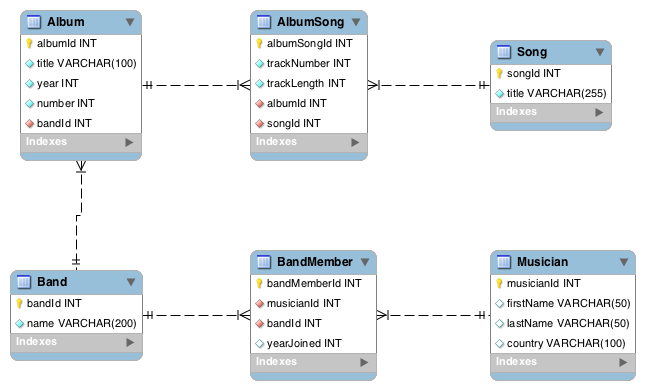
\includegraphics[scale=.650]{images/albums}
\caption{Albums Database}
\label{figure:albumDB}
\end{figure}

Data can be added to a database using \mintinline{sql}{insert} statements 
and existing data in a database can be manipulated using \mintinline{sql}{update}
and \mintinline{sql}{delete} queries.  However, records in a table that may be
referenced by records in other tables via a foreign key cannot be deleted
unless the referencing records are handled first.  Likewise, data that requires
a reference to data in other tables cannot be inserted prior to inserting the
referenced records.  

Complete the first section of your worksheet.

\section*{Altering a Database}

A careful examination of the DDL file provided (\mintinline{text}{albums.sql}) 
indicates how these tables were built and related to each other.  New 
requirements may mean that the underlying data model must be modified to 
support new pieces of data.  For example, if we wanted to keep track of the 
emails of each Musician we could modify the Musicians table to include an 
email address.  SQL allows us to \emph{alter} existing tables using
the following syntax.

\mintinline{sql}{alter table Musician add emailAddress varchar(50);}

A better solution would add support for multiple emails in which case we 
would need to add an entirely new table.

\begin{minted}{sql}
create table Email (
  emailID int not null primary key auto_increment
  musicianId int not null,
  address varchar(100) not null,
  foreign key `fk_email_to_musician` (musicianId) 
    references Musician(musicianId)
);
\end{minted}

In this lab, you will build on the Albums database to add support 
for modeling venues (concert halls) at which bands are under 
contract to play select album songs. You will add tables and keys 
to this database to support this functionality.

\section*{Developing a Solution}

Design entities and relation(s) to extend the Albums database such 
that it supports the following concert information:

\begin{itemize}
  \item The band playing at the concert
  \item The band's select album songs played at the concert
  \item The date the concert was held (use an appropriately formatted 
    \mintinline{sql}{VARCHAR}, date time types are not 
    cross-compatible) 
  \item The name of the hall where the concert was held
  \item The number of seats in the concert hall
  \item The number of concert tickets sold
\end{itemize}

The entities and relations illustrated in Figure \ref{figure:hint} serve as a 
basis for the solution. You will add fields and another entity 
by following the first section of the worksheet.
 
\begin{figure}[h]
\centering
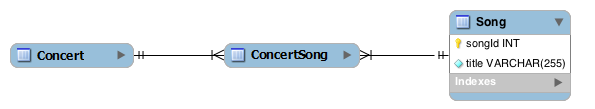
\includegraphics[scale=.50]{images/hint}
\caption{The Song table is part of the original database, relations
between the concert and concert songs are suggested.}
\label{figure:hint}
\end{figure}

The \mintinline{sql}{Song} table is part of the original Albums 
database. Relationships between two entities are indicated by a 
line between the two entities and in general are either a 
one-to-one relationship or a one-to-many relationship.  Figure \ref{figure:example} shows the standard way to draw the two types 
of relations.
 
\begin{figure}[h]
\centering
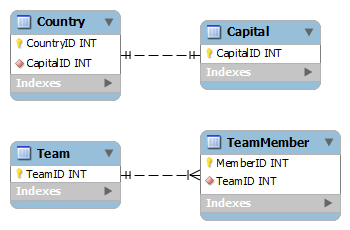
\includegraphics[scale=.50]{images/Example}
\caption{The line connecting the Country entity and the Capital entity describes a one-to-one relation. The line connecting the Team entity with the TeamMember entity describes a one-to-many relation.}
\label{figure:example}
\end{figure}

Complete the first section of the worksheet. 

\section*{SQL Script Modification}

Now that you have properly designed the database modifications, 
you will realize them by writing SQL scripts (or modifying the 
original DDL file, \mintinline{text}{albums.sql}).  Follow the directions in the 
worksheet in order to add the entities and relations you have 
designed in the previous activity to the tables and relations 
in the original Albums database.

\section*{Advanced Activity (Optional)}

Consider the venues listed in Table \ref{table:concertHalls}.

\begin{table}[h]
\centering
\begin{tabular}{l|l}
Venue Name & Capacity \\
\hline\hline
The Mega Dome & 12,000 \\
The Gorge & 32,000 \\
Hotel Concert Hall & 5,000 \\
Cruise Concert Hall & 2,000 \\
\end{tabular}
\caption{The concert halls}
\label{table:concertHalls}
\end{table}

Say that one concert was held at each of the concert halls 
according to the following rules listed bellow. Write an SQL 
script to insert data into the newly designed tables using the 
rules bellow.

\begin{enumerate}
  \item In descending order of concert hall capacity, bands are 
    assigned a concert hall in descending order of the number of 
    their album songs and ascending order of their band name. That 
    means the band with the most number of album songs and the 
    smallest (lexicographically) band name gets the highest capacity 
    concert hall and the band with the second highest number of album 
    songs get the second highest capacity concert hall.
  \item The songs played at each concert are those which have at least 
    one album song of 5 minutes or longer.
  \item Each concert is sold out.
\end{enumerate}

\end{document}
